\documentclass{VUMIFInfBakalaurinis}
\usepackage{algorithmicx}
\usepackage{algorithm}
\usepackage{algpseudocode}
\usepackage{amsfonts}
\usepackage{amsmath}
\usepackage{bm}
\usepackage{caption}
\usepackage{color}
\usepackage{float}
\usepackage{graphicx}
% \usepackage{hyperref}  % Nuorodų aktyvavimas
\usepackage{listings}
\usepackage{subfig}
\usepackage{url}
\usepackage{wrapfig}


% Titulinio aprašas
\university{Vilniaus universitetas}
\faculty{Matematikos ir informatikos fakultetas}
\department{Matematinės informatikos katedra}
\papertype{Baigiamasis bakalauro darbas}
\title{Konvoliucinių neuroninių tinklų tyrimas ir taikymas ranka rašyto teksto atpažinimui}
\titleineng{Research of Convolutional Neural Networks for Handwritting Recognition}
\status{4 kurso studentas}
\author{Ignas Jatulis}
% \secondauthor{Vardonis Pavardonis}   % Pridėti antrą autorių
\supervisor{lekt. Irus Grinis}
\reviewer{-}
\date{Vilnius \\ \the\year}

% Nustatymai
% \setmainfont{Palemonas}   % Pakeisti teksto šriftą į Palemonas (turi būti įdiegtas sistemoje)
\bibliography{bibliografija} 

\begin{document}
\maketitle

\tableofcontents

\sectionnonum{Sąvokų apibrėžimai}

\sectionnonum{Įvadas}
[Iš tiriamojo seminaro, bus perrašyta]
Šiais laikais žmonės vis daugiau veiksmų atlieka kompiuterio pagalba. Pavyzdžiui, jei seniau studentai sesijos metu, prieš egzaminus, konspektus rašydavo ranka, tai šiais laikais, vis daugiau studentų renkasi kompiuterį, jame esančias teksto rengykles, kurių pagalba galima patogiai ir tvarkingai parengti konspektus. Tačiau sudarydami konspektus iš ranką rašytų sąsiuvinių, jie sugaišta nemažai laiko.  Laiko sutaupymui labai padėtų ranka rašyto teksto atpažinimo programėlė. Šiam tikslui pasiekti, pasitelksime vieną populiariausių kompiuterinės regos bibliotekų OpenCV ir sukonstruotą dirbtinį neuronų tinklą.

Taigi, šiame baigiamojo bakalauro darbe panagrinėsime ranka rašyto teksto atpažinimo galimybes, panagrinėsime kokie yra pradinių duomenų šaltiniai, kokiu tikslumu pavyks atpažinti ranka parašytą tekstą.

\section{Darbo uždaviniai}
\begin{enumerate}
    \item Susipažinti su konvoliucinių neuroninių tinklų taikymu ranka rašyto teksto atpažinimui
    \item Susipažinti su konvoliucinių neuroninių tinklų architektūromis, įrankiais jų konstravimui;
    \item Susirasti pradinių duomenų bazę;
    \item Sukurti programos prototipą, kuri leistų panagrinėti konvoliucinių neuroninių tinklų apmokymo rezultatus, atpažinti ranka parašytą tekstą. 
\end{enumerate}

\section{Teorija}

\subsection{Teksto atpažinimas}
Teksto atpažinimo rūšys (Optical character recognition (OCR), Intelligent character recognition (ICR), Intelligent word recognition (IWR))
Kokios problemos kylą atpažįstant tekstą, istorija, ką pavyko pasiekti, kokia įrankiai egzistuoja dabar.

http://cs231n.stanford.edu/reports/2017/pdfs/810.pdf
https://pdfs.semanticscholar.org/3c6d/38e010a3334ca76f3a5ddba31e2c540e9a18.pdf
https://cs.stanford.edu/~acoates/papers/wangwucoatesng_icpr2012.pdf
https://towardsdatascience.com/handwriting-recognition-using-tensorflow-and-keras-819b36148fe5


\subsection{Prižiūrimasis mokymas}

Pagrindinė mašininio mokymosi forma konvoliuciniuose neuroniniuose tinkluose yra prižiūrimasis mokymasis (angl. supervised learning). Prižiūrimasis mokymas yra mašininio mokymo viena iš krypčių. Šis metodas analizuoja pateiktus didelės apimties pradinius duomenų kiekius ir konstruoja numanomą funkciją, kurį gali būti naudojama naujų reikšmių klasifikavimui, kurias vėliau nustatytume naudojimo metu. Kiekvienai pradinių duomenų kategorijai yra priskiriamos etiketės (angl. labels). Tarkim, mūsų atveju, turint "A" ranka rašytos raidės pradinių duomenų grupę, suteikiame jiems A etiketę, raidės "B" duomenų grupei suteikiame B etikete ir taip toliau. Paprastai, prižiūrimojo mokymo metu yra naudojama didelės apimties duomenų grupės. Mokymo metu, kaip įvestis yra naudojami vaizdai ir jų etiketės. Mokymo iteracijų metu yra gaunami rezultatai, kiek tiksliai pradinių duomenų buvo tiksliai priskirti galutinei reikšmei, yra apskaičiuojamos klaidos tikimybės funkcijos, pakeičiami kintami parametrai, kurie yra neuronų svoriai, taip, kad būtų sumažinta klaidos tikimybė, duomenų klasifikacijai, kito žingsnio metu. Paprastai, tokio mokymo paremtose sistemose būna milijonai keičiamo svorių, kurie ieškomi apmokant neuroninį tinklą. Tam atlikti, praktikoje dažnai naudojama yra SGD (angl. stochastic gradient descent) procedūra, kurios vykdymo metu ir yra modifikuojami svoriai. Be stochastinio gradiento aproksimacijos metodo, taip pat yra naudojami gradiento aproksimacijos bei antros eilės gradiento aproksimacijos metodai.

[O. Bousquet and L. Bottou, "The Tradeoffs of Large Scale Learning," in Advances in Neural Information Processing Systems 20, Curran Associates, Inc., 2008. ]
 
Prižiūrimojo mokymosi pabaigoje yra tikrinamas apmokyto neuroninio tinklo tikslumas, naudojant kitą, neuroniniam tinklui prieš tai nematytą, testinę duomenų grupę, kurios dalys nebuvo panaudotos pradinių duomenų rinkinyje. Universalumas rezultatams yra labai svarbus veiksnys. Pavyzdžiui ranka rašyto teksto atpažinime, gali skirtis ieškomos raidės pozicija vaizde (pavyzdžiui ne centre), raidės pavirtimo kampas, pašalinis triukšmas fone.

Problemų sprendimo žingsniai naudojant prižiūrimąjį mokymą:
\begin{enumerate}
  \item Reikia nusistatyti kokie bus pradiniai duomenys, kuriais apmokysime tinklą. Pavyzdžiui, ranką rašyto teksto atpažinimui, galime panaudoti atskirai ranką rašytų raidžių duomenų rinkinius arba pilnai parašytų žodžių duomenų rinkinius.
  \item Pradinių duomenų rinkinio sudarymas. Duomenų rinkinys turi atspindėti realiame gyvenime naudojamus duomenis.
  \item Pradinių duomenų paruošimas apmokymui. Modelio tikslumas smarkiai priklauso nuo pradinių duomenų rinkinio. Paprastai, duomenys apvalomi nuo foninio triukšmo, išryškinamos jų savybės, transformuojamos į patogius apmokymui objektus, pavyzdžiui vektorius, kurie nusako mokomo objekto savybes. Savybių skaičius neturi būti per didelis, bet tuo pačiu ir ne per mažas, kad užtektų pradinės informacijos tikslaus rezultato nustatymui.
  \item Mokymo struktūros ir algoritmų pasirinkimas. Pavyzdžiui Atraminių vektorių klasifikavimas, neuroniniai tinklai ar kiti algoritmai ir jų junginiai.
  \item Modelio apmokymas naudojant pradinių duomenų rinkinį. Kai kurie prižiūrimojo mokymosi algoritmai reikalauja, kad vartotojas nustatytų tam tikrus valdymo parametrus. Šie parametrai gali būti koreguojami, pavyzdžiui atliekant kryžminį patvirtinimą.
  \item Įvertinti apmokyto modelio tikslumą. Po parametrų sureguliavimo ir mokymosi rezultatų tikslumas turi būti matuojamas testinių duomenų rinkiniu, kuris nebuvo naudojamas pradinių duomenų rinkinyje.
\end{enumerate}

\subsection{Konvoliuciniai neuroniniai tinklai}
Šiuo metu viena pagrindinių giliojo mokymo panaudojimo sričių yra vaizdinių objektų atpažinimas. Nuolatos yra vykdomi tyrimai, kaip pagerinti mašininio mokymosi metodus, taip pat naudoti vis didesnes duomenų grupes, naudoti tinkamesnes technikas, saugantis nuo duomenų perderinimo (angl. overfitting) [8]. Jeigu tinklo mokymo metu yra pasiekiamas didelis tikslumas, tačiau patikros tikslumas toliau sekančių iteracijų metu išlieka žemas, tai reiškia, jog neuroninis tinklas yra perderinamas – neuroninis tinklas mokosi tokius objekto požymius, kurie nepadeda ar trukdo klasifikuoti objektus į klases. Perderinimo problema yra sprendžiama stabdant mokymo procesą, kai mokymo duomenų grupės naudojimo metu, neuroninio tinklo klasifikavimo tikslumas pradeda blogėti tolesnių iteracijų metu, taip pat yra naudojamos nuobaudos neuroninio tinko svoriams bei išmetimo operacijos. Konvoliucinai neuroniniai tinklai yra specialus duomenų apdorojimo būdas, įsivaizduojamas, kaip tinklelio tipo topologija. Pavadinimas, konvoliuciniai neuroniniai tinklai nusako, kad tinklo apmokymo metu yra bent vieną kartą naudojama matematinė operacija, vadinama konvoliucija [3]. Konvoliuciniai neuroniniai tinklai naudojasi bendrais duomenų svoriais, taip mažindami parametrų, kuriuos kompiuteris turi išmokti iš duomenų, kiekį, taip pat yra sumažinamas mokymo laikas bei sunaudojami ištekliai neuroninio tinklo apmokymo procesui. Tarp neuroniniuose tinkluose naudojamų parametrų vienas svarbiausių yra vadinamas mokymosi greičiu (angl. learning rate), kurio pasirinkimas daro įtaką efektyviam pajėgumo kontroliavimui, optimizavimo greičiui. Efektyvus neuroninio tinklo pajėgumas yra pats geriausiais, kai mokymosi greitis yra teisingiausiai parenkamas optimizavimo problemai spręsti. Esant mažam mokymosi greičiui yra pasiekimas didžiausias tikslumas, tačiau yra ilginamas mokymosi laikas. Pasirinkus per mažą tinklo mokymosi greitį optimizavimui, mokymosi procesas ne tik užtrunka ilgiau, siekiant optimalaus rezultato, bet gali įstrigti, dėl didelio mokymosi klaidų kiekio [3]. Taip pat šiuose neuroniniuose tinkluose yra naudojami telkimo (angl. pooling) sluoksniai, tam kad būtų sumažinami gaunamos informacijos matmenys, jais naudojantis architektūra yra paverčiama į mažiau jautrią įvairių veiksnių poveikiui perduodamuose duomenyse [9]. Siekiant įgyvendinti išsikeltus uždavinius, yra modeliuojamos sluoksnių hierarchijos bei duomenų apdorojimui reikalingos savybės, tokios kaip filtravimo tinklelio dydis, filtro žingsnio dydis bei išeigos gylis. Dabartiniuose neuroniniuose tinkluose į klasifikatorių yra perduodama visų prieš tai buvusių sluoksnių išeiga, grafo tipo rinkinys. Bendra tinklo kūrimo idėja yra į kiekvieną sekantį sluoksnį, perduodant prieš tai buvusių sluoksnių rinkinį. Naudojantis šia metodika tinklas paruošiamas atpažinti ne tik aukšto lygmens (angl. high-level) požymius, bet ir mažas, tikslias detales, filtravimo būdu atskiriant iš duomenų žemo lygmens (angl. low-level) požymius, kurie yra mažiau kintantys tam tikrose klasėse, taip aptinkant pagrindinius klasę nusakančius motyvus [2]. Pagrindinis sistemų, naudojančių neuroninius tinklus giliajam mokymui tikslas yra kuo aukštesnis testavimui skirto duomenų rinkinio rezultatas. Esant žemai mokymo klaidos tikimybei, siekiant pagerinti patį pagrindinį rezultatą, galima surinkus, transformavus daugiau duomenų. [3]

\subsubsection{Konvoliucijos operacija}
Kiekviename konvoliuciniame neuroniniame tinkle yra bent viena konvoliucijos operacija.  Šios operacijos rezultatas dažnai yra vadinamas požymių žemėlapiu (angl. feature map). Konvoliucijos sluoksnio parametrai yra sudaryti iš mokomųjų filtrų (angl. learnable filters) rinkinio. Filtro pozicijos keitimo metu yra skaičiuojama skaliarinė filtro elemento bei perduotų duomenų svorių sandauga, taip yra sukuriamas dviejų dimensijų dydžio aktyvacijos žemėlapis. Visas konvoliucinio sluoksnio rezultatas – požymių žemėlapių rinkinys Šių aktyvacijos žemėlapių dėka neuroninis tinklas yra išmokomas atpažinti tam tikrus požymius, kaip objektų briaunas,  regionus, kuriuose dominuoja tos pačios sąvybės [3]. 

\begin{figure}[H]
    \centering
    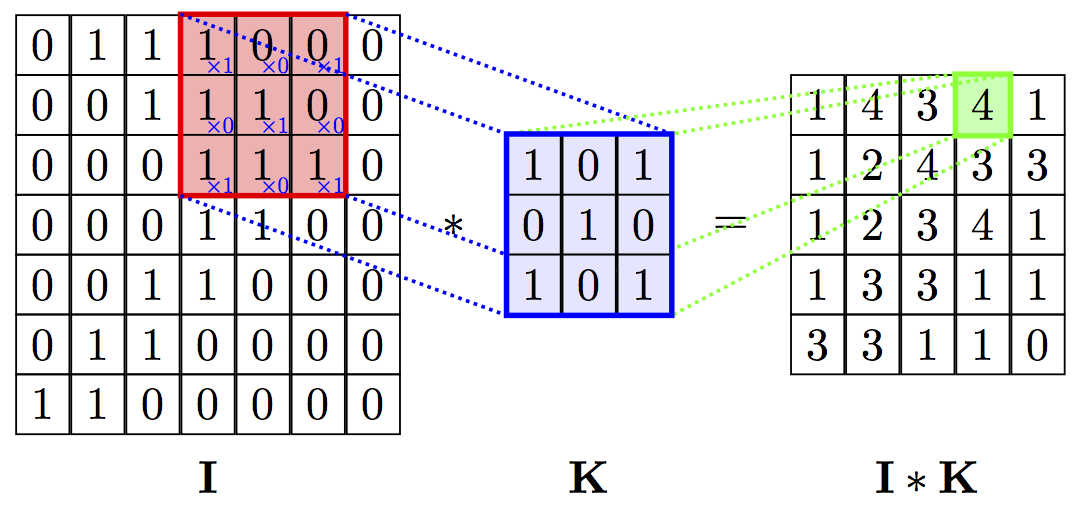
\includegraphics[scale=1.5]{img/konvoliucija.png}
    \caption{Konvoliucijos operacija}
    \label{img:emnist_sudarymas}
\end{figure}

\subsubsection{ReLU normalizacijos funkcija}
Po kiekvieno konvoliucijos sluoksnio, neuroniniuose tinkluose yra naudojamos aktyvacijos funkcijos. Kompiuteriniuose vaizduose, siekiant duomenų normalizacijos, populiariausia yra ReLU aktyvavimo funkcija, kuri yra įvardijama, kaip geriausiai tinkanti neuroninio tinklo mokymo efektyvumui. Ši funkcija yra naudojama, kaip max(0, x) [10], x šiuo atveju yra konvoliucijos operacijos rezultatas dvimatės matricos elementui [14]. Kitaip tariant, visos, neigiamos požymių žemėlapio reikšmės, po konvoliucijos operacijos, yra paverčiamos į 0. 
\subsubsection{Sutelkimo funkcija}
Pagrinde konvoliuciniuose neuroniniuose tinkluose yra naudojamos maksimalaus telkimo, vidutinio telkimo operacijos. Pasirinkta operacija yra naudojama tarp konvoliucinių sluoksnių. Telkimo operacija progresyviai mažina reprezentacijos dydį, ko rezultate yra mažinamas parametrų bei skaičiavimų skaičius, reikalingas neuroninio tinklo apmokymui. Naudojantis telkimo operacija požymių žemėlapių skaičius nekinta. Naudojantis bet kuria iš šių operacijų, kuriama objektų reprezentacija, kuri tampa beveik nekintama, pagal mažus pradinių duomenų skirtumus. Atsižvelgus į tai, telkimo operaciją galima naudoti tada ir tik tada, kai siekiama, mažo jautrumo įvairiems požymiams. Pasitvirtinus prielaidai, telkimo operacijų naudojimas padidina neuroninio tinklo statistinį efektyvumą. Naudojant telkimo operaciją po parametrizuotų konvoliucijos operacijų, yra pasiekiami ir išmokstami nekintantys požymiai. Maksimalaus telkimo operacijos metu, naudojant pasirinktą stačiakampio formos filtrą bei pasirenkant pačią didžiausią reikšmę filtro viduje, tuo tarpu vidutinio telkimo operacijos metu, pasirinkto  filtro viduje yra apskaičiuojamas reikšmių vidurkis. Praktikoje, dėl tinkamesnių rezultatų plačiausiai naudojama maksimalaus telkimo operacija [3]. 

\subsubsection{Pilnai sujungti sluoksniai}
Pilnai sujungti sluoksniai yra labai panašūs į konvoliucinius sluoksnius. Vienintelis jų skirtumas yra toks, kad neuronai, konvoliuciniuose sluoksniuose yra sujungti tik su lokaliais regionais pradiniuose duomenyse bei jie tarpusavyje  naudojasi padalintais parametrais. Abiejuose sluoksniuose yra naudojama skaliarinė sandauga. Taip pat pilnai sujungtą sluoksnį galima konvertuoti į konvoliucinį sluoksnį. Pavyzdžiui, jeigu duomenys į pilnai sujungtą sluoksnį perduodami 7x7x512 dimensijomis, o siekiamas - 4096 neuronų skaičius pilnai sujungtame sluoksnyje, rezultatui pasiekti galima naudoti konvoliucijos operaciją, kaip parametrus naudojant 7x7 dimensijų dydžio filtrą, 1 pikselio dydžio filtro žingsnį bei išeities (požymių žemėlapio) gylį lygų 4096 [15]. 

\subsection{Konvoliucinių neuroninių tinklų architektūros}

Žemiau esančiuose skyriuose panagrinėsime naudojamas konvoliucinių neuroninių tinklų architektūras.

\subsubsection{LeNet}

LeNet architektūra pirmą kartą buvo pristatyta 1998 metais. Ši architektūra buvo pritaikyta skaitiniam atpažinimui. Kadangi tuo metu grafikos apdorojimo įrenginiai iš tolo neprilygo dabartiniams produktams, buvo  labai svarbu, kad apdorojant sluoksniuose esančius svorius bei juos saugant  užtektų turimų išteklių. Kaip sprendimas buvo pasiūlyta 7 sluoksnių architektūra (žr. 4 pav.), kurios pradiniai duomenys, vaizdai  yra 32x32 dydžio. Ši architektūra buvo skirta skaitinių vaizdinių identifikavimui, tokių, kaip pašto kodų ar skaičių atpažinimui. Pagrindinė šio neuroninio tinklo architektūros idėja buvo – po kiekvieno konvoliucinio sluoksnio, turi būti telkimo sluoksnis, todėl šioje architektūroje yra 2 konvoliuciniai, 2 maksimalaus telkimo bei 3 pilnai sujungti sluoksniai [15].  Y. LeCun, "Gradient-based learning applied to document recognition," in Proceedings of the IEEE 86.11, 1998.  
[

https://www.ibm.com/developerworks/library/cc-machine-learning-deep-learning-architectures/index.html

\subsubsection{AlexNet}
AlexNet architekūra buvo pristatyta 2012 metais rengtame ImageNet konkurse, kurio tikslas buvo sukurti sprendimą, kurio dėka būtų suklasifikuojami 1.2 milijono didelės raiškos vaizdų į 1000 skirtingų klasių. Šios architektūros idėja yra pakeisti patobulinti LeNet kurtą architektūrą, įrodant, kad telkimo operacija neturi būti atliekama kas kartą po konvoliucijos operacijos. AlexNet architektūrą iš viso sudaro 11 sluoksnių su svoriais, iš jų 5 yra konvoliuciniai sluoksniai, 3 – maksimalaus kaupimo sluoksniai, o likę 3 – pilnai sujungti sluoksniai. Kaip pradinis duomuo buvo perduodamas 224x224x3 dydžio paveikslėlis, su 96 11x11x3 dydžio filtrais (angl. kernel) su 4 pikselių didžio filtro žingsniu. [8]  
 
 A. Krizhevsky, I. Sutskever and G. E. Hinton, "ImageNet Classification with Deep Convolutional Neural Networks," Curran Associates, Inc., 2012, pp. 1097-1105
 
\subsubsection{ResNet}

\section{Panaudoti įrankiai}
\subsection{Vaizdo apdorimas}
Nuotraukų apdorojimui buvo pasirinkta OpenCV biblioteka ([2]). OpenCV (Open Source Computer Vision Library) yra atvirojo kodo kompiuterinės regos biblioteka. Šią biblioteką galima naudoti tiek mokslo, tiek komercijos tikslais. „OpenCV“ pradėta kurti vieno iš „Intel“ bendrovės padalinio 1999 metais. Šiuo metu „OpenCV“ labiausiai plėtoja ir palaiko kompiuterinę regą tyrinėjanti bendrovė „Itseez“. Kadangi biblioteka yra atvirojo kodo, jos išeities kodą galime surasti GitHub.com([1]) saugykloje, todėl prie jos tobulinimo ir kūrimo gali prisidėti kiekvienas.

„OpenCV“ kompiuterinės regos bibliotekoje yra realizuota daugiau kaip 2500 optimizuotų algoritmų kurie padeda apdirbti vaizdus. Originaliai ši biblioteka buvo parašyta su C++ kalba, tačiau ji taip pat turi sąsajas tokioms populiarioms programavimo kaip Python, JAVA ar MATLAB programiniai įrangai. Taip pat, ji yra suderinama su populiariausiomis operacinėmis sistemomis, tokiomis kaip Windows, Linux, Android ar Mac OS. Apie kiekvieną bibliotekoje esantį algoritmai ir jo panaudojimo pavyzdžius, galima rasti OpenCV dokumentacijoje ([1]).
\subsection{KNT konstravimo karkasas}

Parašyt apie Keras, kokie buvo kiti pasirinkimai, bet kodėl Keras (dėl paprastumo jo ir palaikomo API).

\subsection{Programavimo aplinka ir priemonės}
Klasifikavimo metodų tyrimui atlikti buvo naudojamas ASUS X550LB nešiojamasis kompiuteris su Intel® Core™ I7-4500U dviejų branduolių 1.80 GHz procesoriumi. Kompiuteryje yra naudojama 8 GB dydžio operatyvioji atmintis. Taip pat bandymų aplinkoje buvo įdiegta Ubuntu 16.4 operacinė sistema

\subsection{Pradinių duomenų bazė}

[Dar viena buvo: http://www.ee.surrey.ac.uk/CVSSP/demos/chars74k/ bet tik ~3500 raidžių pavyzdžių, esant teksto trukumui, galima panaudot].

Konvoliucinių neuroninių tinklų apmokymui buvo nuspręsta naudoti EMNIST ranką rašytų raidžių duomenų bazę \cite{Emnist}. 

\begin{figure}[H]
    \centering
    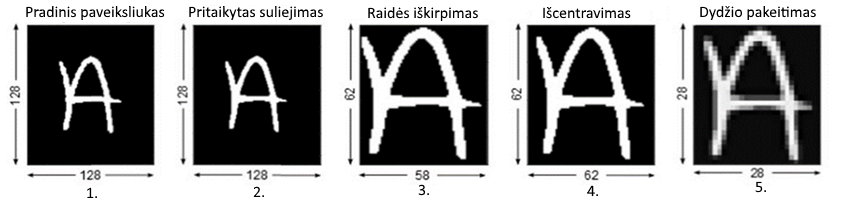
\includegraphics[scale=1.5]{img/emnist_sudarymas.png}
    \caption{Pradinių duomenų paruošimas}
    \label{img:emnist_sudarymas}
\end{figure}

Šį duomenų bazė buvo sudaryta pertvarkant NIST Special Database 19. Kaip buvo pertvarkomi duomenys iliustruota aukščiau esančiame "Pradinių duomenų paruošimas" paveiksliuke. Originalus paveikslėlis buvo 128 x 128 pikselių dydžio (1.) Buvo pritaikytas Gauso filtro suliejimas, kad būtų paapvalinami kampai (2.). Jei simbolis neužima viso paveiklėlio ploto, jis yra iškerpamas (3.) ir sucentruojamas (4.) paliekant 2 pikselių paraštes nuo simbolio krašto. Galiausiai paveikslėlis normalizuojamas į 28 x 28 pikselių dydžio, juodai baltą vaizdą.

Šis duomenų rinkinys yra išskaidytas į šešias dalis. Trumpas šių dalių aprašymas, iš ko susideda:
\begin{itemize}
    \item EMNIST ByClass: 814255 simboliai. 62 nesubalansuotos klasės;
    \item EMNIST ByMerge: 814255 simboliai. 47 nesubalansuotos klasės;
    \item EMNIST Balanced:  131600 simbolių. 47 subalansuotos klasės;
    \item EMNIST Letters: 145600 simbolių. 26 subalansuotos klasės;
    \item EMNIST Digits: 280000 simbolių. 10 subalansuotos klasės;
    \item EMNIST MNIST: 70000 simbolių. 10 subalansuotos klasės;
\end{itemize}
    


\subsection{Pasirinkta KNT architektūra}

\section{Rezultatai}

\subsection{Teksto skaidymas}
\subsubsection{Eilutėmis}
\subsubsection{Žodžiais}
\subsubsection{Atskiromis raidėmis}
\subsubsection{Naudojant rėmelį}

\subsection{Konvoliucinio neuroninio tinklo konstravimas}

Nuotrauka, kaip kode atrodo
Rezultatų lentelė, kaip keitėsi skirtingų duomenų kiekių, skirtingais epochų skaičiais, tikslumas ir kiek kas trūko įsivykdyti.


% tablesgenerator.com - converts calculators (e.g. excel) tables to LaTeX
\begin{table}[H]\footnotesize
  \centering
  \caption{Lentelės pavyzdys}
  {\begin{tabular}{|l|c|c|} \hline
    Algoritmas & $\bar{x}$ & $\sigma^{2}$ \\
    \hline
    Algoritmas A  & 1.6335    & 0.5584       \\
    Algoritmas B  & 1.7395    & 0.5647       \\
    \hline
  \end{tabular}}
  \label{tab:table example}
\end{table}



\sectionnonum{Išvados}
Išvadose ir pasiūlymuose, nekartojant atskirų dalių apibendrinimų,
suformuluojamos svarbiausios darbo išvados, rekomendacijos bei pasiūlymai.

\printbibliography[heading=bibintoc] % Literatūros šaltiniai aprašomi
% bibliografija.bib faile. Šaltinių sąraše nurodoma panaudota literatūra,
% kitokie šaltiniai. Abėcėlės tvarka išdėstoma tik darbe panaudotų (cituotų,
% perfrazuotų ar bent paminėtų) mokslo leidinių, kitokių publikacijų
% bibliografiniai aprašai (šiuo punktu pasirūpina LaTeX). Aprašai pateikiami
% netransliteruoti.
Citavimo pavyzdžiai: cituojamas vienas šaltinis \cite{PvzStraipsnLt}; cituojami
keli šaltiniai \cite{PvzStraipsnEn, PvzKonfLt, PvzKonfEn, PvzKnygLt, PvzKnygEn, PvzElPubLt, PvzElPubEn, PvzMagistrLt, PvzPhdEn}.

\sectionnonum{Santrauka}
Šiame darbe buvo tiriamas konvoliucinių neuroninių tinklų pritaikymas ranka rašyto teksto atpažinimo problemos sprendimui. Bakalauriniame darbe aprašomos pagrindinės operacijos ir technikos vaizdų klasifikacijai ir atpažinimui naudojant konvoliuciniuos neuroninius tinkluose. Taip pat šiame darbe aprašomi kelio ženklų atpažinimui skirti duomenų rinkiniai bei tų rinkinių problemos, darančios įtaką galutiniams giliojo mokymo rezultatams. Darbe yra apžvelgiamos populiariausios egzistuojančios technologijos – karkasai, skirti atvaizdų klasifikacijos problemai spręsti. Darbe yra lyginamos panašių problemų sprendimui naudotos architektūros, skirtos modeliuoti konvoliucinius neuroninius tinklus, bandymu metu vertinami jų pasiekti rezultatai. 
Raktiniai žodžiai: teksto atpažinimas, konvoliuciniai neuroniniai tinklai, prižiūrimasis mokymas.

\sectionnonum{Summary}


\end{document}